\chapter{Model Validation and Hardware}\label{ch:validation}

\section{Three independent implementations of the same physics}

The broadcast channel model gives the saturation bound $N_{\mathrm{sat}}$ of \Cref{ch:codesign}
and was the input to the envelope that chapter used to report, so it is validated against two
independent sources and not one.

\begin{table}[h]
\centering
\caption{Saturation throughput (Mb/s), $1400$\,B broadcast frames. The slot-exact simulator was
written \emph{before} the published model was located and shares none of its assumptions.}
\label{tab:validation}
\begin{tabular}{rrrrrr}
\toprule
$N$ & published model & slot-exact sim & $\Delta$ & NS-3 & $\Delta$ \\
\midrule
5  & 4.3329 & 4.3305 & $-0.06\%$ & 4.3318 & $-0.03\%$ \\
10 & 3.1319 & 3.1321 & $+0.00\%$ & 3.1288 & $-0.10\%$ \\
20 & 1.7823 & 1.7830 & $+0.04\%$ & 1.7866 & $+0.24\%$ \\
35 & 1.2407 & 1.2407 & $-0.00\%$ & 1.2343 & $-0.51\%$ \\
50 & 1.2595 & 1.2585 & $-0.08\%$ & 1.2541 & $-0.43\%$ \\
\bottomrule
\end{tabular}
\end{table}

Agreement is $\leq 0.08\%$ against the independent simulator and $\leq 0.51\%$ against NS-3. Unicast
agrees with the acknowledged DCF model to $-\valUniLo$/$+\valUniHi\%$ across $N = 5$--$50$, with fixed-point
residuals below $10^{-12}$.

\begin{figure}[h]
\centering
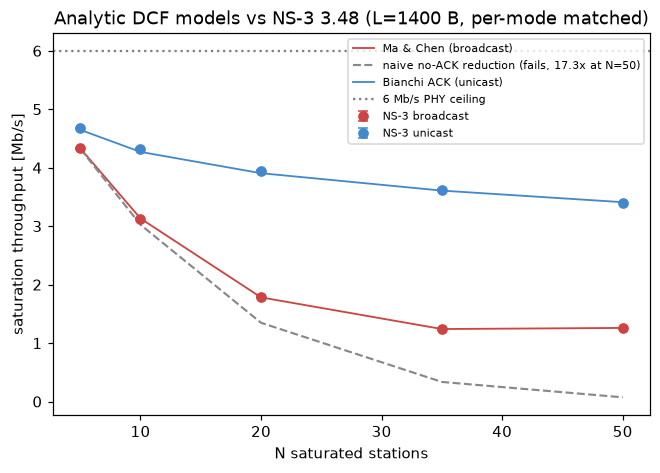
\includegraphics[width=0.75\textwidth]{fig_ns3_bianchi.png}
\caption{Analytic models against simulation, both modes.}
\label{fig:validation}
\end{figure}

\section{The mechanism, confirmed by removing it}

The reason broadcast needs its own model is a specific asymmetry. A station that has just
transmitted redraws its backoff and may draw zero, taking the medium immediately after the
interframe space, while every station that deferred necessarily holds a counter of at least one. In
unicast the acknowledgement timeout blocks colliders from doing this; in broadcast nothing does.

The slot-exact simulator can disable \emph{exactly} that asymmetry and nothing else. Doing so
collapses it onto the naive reduction --- a $16.9\times$ gap at $N = 50$. \textbf{The mechanism
attribution is therefore not an inference from agreement; it is a controlled intervention.}

\begin{remark}[An expensive lesson]
This project used the naive reduction --- the unicast model with the acknowledgement removed and
the transmission probability fixed --- for several phases. It under-predicts by $16\times$ at
$N = 50$. The published broadcast model's own authors open by warning that unicast models cannot
simply be reduced for broadcast analysis. \emph{The failure was reading a model without reading its
preamble.}
\end{remark}

\section{A non-monotonicity that is real}

Saturation throughput is \textbf{not monotone decreasing} in $N$: it dips near $N \approx 35$ and
recovers. All three implementations reproduce it, so it is a property of the freeze-process series
rather than a bug --- each freeze stage contributes a hump peaking at a station count set by the
contention window.

This matters operationally. The capacity search breaks on the first violating $N$, which is valid
only if utilisation is monotone. It is --- because the explicit factor $N$ in the numerator outruns
the recovery --- but \textbf{that is an arithmetic accident, not a structural guarantee}, and it is
now verified exhaustively rather than assumed.

\section{Hardware}\label{sec:hardware}

Two Raspberry Pi 4 boards in ad hoc mode on a $5$\,GHz channel, broadcasting $1400$\,B frames at
$6$\,Mb/s. Four things were measured on them: the loss of the link, how one radio spaces its
own frames, the loss when both send at a set load, and the loss when both always have a frame
to send. The second and the fourth were not planned. They are what the third made necessary.

\subsection{The link}

With one transmitter at $100$ frames/s, \hwLossFrames{} frames of \hwSentFrames{} were lost in
August 2026 ($p = \hwLoss$), and none of \hwSentFrames{} when the same session was repeated in
October. This is the loss of a link with no contention.

\begin{remark}[A figure withdrawn]
Earlier versions of this chapter and of the paper reported ``airtime $1.995$\,ms per frame
against $1.988$\,ms predicted, a gap of $0.36\%$'', and called it an independent check on the
timing constants. Both figures were wrong, in opposite senses. The measured one was the rate at
which the sender's operating system accepted frames, which counts those still queued when the
sender stops; on air the frames were \hwCycleOn\,ms apart. The predicted one left out the
$64$\,B of headers every frame carries and assumed the standard's backoff; the standard's
figure is \hwCycleStd\,ms. An agreement of $0.36\%$ did not invite a second look, and for two
months it did not get one.
\end{remark}

\begin{remark}[A warning earned earlier]
An initial $2.4$\,GHz sweep produced a tidy $97.45\%$ delivery figure that was \textbf{saturation
at the 802.11b $1$\,Mb/s broadcast basic rate}, not channel loss. It was caught by a pre-stated
prediction plus a load sweep, and is kept in the record labelled as what it was. Repeatability did
not protect against it --- the standard deviation across windows was small. \emph{A precisely
reproducible measurement of the wrong thing looks exactly like a good measurement.}
\end{remark}

\subsection{How one radio spaces its own frames}\label{sec:spacing}

A saturated station that keeps to the standard sends a frame, waits DIFS, counts a number of
slots drawn from $0$ to $15$, and sends the next: for this frame \hwCycleStd\,ms from one frame
to the next, of which \hwGapStd\,\si{\micro\second} is the gap. A receiver can measure that time
without any help from the sender: the sequence numbers it spans, over the time from the first
frame it hears to the last (\Cref{tab:spacing}).

\begin{table}[ht]
\centering
\caption{Time from one frame of a saturated sender to its next, read at the receiver. The frame
itself is $1976$\,\si{\micro\second} on air.}\label{tab:spacing}
\begin{tabular}{lrr}
\toprule
 & per frame (ms) & gap (\si{\micro\second}) \\
\midrule
the standard's rule                                   & \hwCycleStd & \hwGapStd \\
this radio, the driver's settings (August and October) & \hwCycleOn  & \hwGapOn \\
this radio, the vendor's frame-burst mode off          & \hwCycleOff & \hwGapOff \\
\bottomrule
\end{tabular}
\end{table}

\textbf{The radio does not keep the standard's rule between its own consecutive frames.} The
Linux driver switches the chip's \emph{frame-burst} mode on whenever it configures
it~\cite{linuxframeburst}; with that mode off the spacing moves toward the standard's and stops
short of it. This is not peculiar to one chip: Bianchi \emph{et al.} measured the same quantity
on six commercial cards, with an instrument built for the purpose, and found that none of them
kept to the standard~\cite{bianchi2007cards}. The firmware is closed. What it does is inferred
here from a mean spacing; no single frame was timed.

\subsection{Two radios at a set load: the registered experiment}\label{sec:contention-hw}

What two boards can test is the mechanism the capacities are made of: the loss among stations
that all send, at a known offered load. Every board sends one frame per period at a redrawn
instant and counts what it receives from the other. The model of \Cref{sec:why} was asked for
its predictions in advance: with two boards filling half, seven tenths and $85\%$ of the medium,
losses of $0.29$, $0.64$ and $1.40\%$; with three, $0.66$, $1.52$ and $3.00\%$
(\Cref{app:prereg}). The band registered for two boards was $0.6$ to $1.4$ times the model's
loss. The two-board case is sharp in one respect: the only receiver of a frame is the other
transmitter, so no third radio can capture one of two colliding frames. ns-3 was run at the
same points first: it agrees with the model within $5\%$ at three to five nodes and is
$9$--$18\%$ below it at two, a small bias of the model at the smallest network that nothing so
small had exposed.

The session was run with two boards on the day it was registered: twelve windows, all of them
usable. \textbf{The prediction held at the first two loads and failed at the third}, where the
radios lost \hwContHighRatio{} of what the model predicts (\Cref{tab:contention-hw}). Loss rises
with load, as predicted, and the two directions lose nearly the same number of frames in every
window, which is what collisions between two half-duplex radios do and what a lossy link does
not.

\begin{table}[ht]
\centering
\caption{Frames lost between two radios, in percent. Three sessions of twelve windows on one
night; the last column is all \hwPoolWindows{} windows over the model's prediction.}
\label{tab:contention-hw}
\begin{adjustbox}{max width=\linewidth}
\begin{tabular}{rrrrrrrr}
\toprule
medium & predicted & registered band & registered & frame burst & repeat & all & over the \\
filled &           &                 & session    & off         &        & windows & model \\
\midrule
$0.50$ & $0.29$ & $0.19$--$0.40$ & \hwContLow  & \hwOffLow  & \hwRepLow  & \hwPoolLow  & \hwPoolLowRatio \\
$0.70$ & $0.64$ & $0.39$--$0.89$ & \hwContMid  & \hwOffMid  & \hwRepMid  & \hwPoolMid  & \hwPoolMidRatio \\
$0.85$ & $1.40$ & $0.85$--$1.95$ & \textbf{\hwContHigh} & \textbf{\hwOffHigh} & \hwRepHigh & \hwPoolHigh & \textbf{\hwPoolHighRatio} \\
\bottomrule
\end{tabular}
\end{adjustbox}
\end{table}

\paragraph{A follow-up in which all four predictions failed.} The spacing of
\Cref{sec:spacing} suggested a cause: a radio that sends its queued frames one behind another,
without contending again, would be described well at low load and lose less than the model at
high load. Four predictions were registered before any run with frame burst off
(\Cref{app:prereg}). One saturated sender would then take $2.070$--$2.095$\,ms per frame: it took
\hwCycleOff. Two boards would then fall inside the original bands: at the highest load they lost
\hwOffHigh\%, under a band that begins at $0.848\%$. A repeat of the first session, frame burst
on, would agree with it: at the highest load it gave \hwRepHigh\% where the first had given
\hwContHigh. And the loss with frame burst off would be at least $1.5$ times the loss with it
on: against the repeat it is no larger at all.

The repeat is what this follow-up was worth. After the run with frame burst off the author was
ready to write that the vendor mode explained a third of the shortfall. \textbf{Frame burst
changes one sender's spacing and has no demonstrated effect on the loss between two boards};
the difference that would have been reported was the scatter between sessions. That scatter is
itself larger than was assumed: \hwPoolSdHigh{} percentage points between windows at the highest
load, where frames lost in independent pairs would give $0.13$.

\paragraph{What the design could not separate.} Two boards can fill the medium only if each
sends often. At $85\%$ each board sends a frame every $4.7$\,ms and its frame lasts $2$\,ms, so
a board frequently holds two frames of its own, and how a radio sends its own queued frames
matters as much as how two radios contend. At the operating point of this thesis ---
\nmaxLeanDesign{} stations, each sending $12.5$ frames a second --- a station almost never holds
two. Below saturation, then, a two-board experiment mixes two things, and the capacities depend
on one of them.

\subsection{Two saturated radios}\label{sec:saturated-hw}

The case that isolates the contention is the one every treatment of the access rule begins
with: both stations always have a frame to send. It needs nothing from a traffic generator. It
was registered before its runs, together with the author's own expectation, which was that the
shortfall belonged to the contention and that about $7\%$ of frames would be lost.

\begin{table}[ht]
\centering
\caption{Two radios, each offered $400$ frames/s where the medium carries about $490$. Frames
on air are read at the receiver. Eight values per column.}\label{tab:saturated-hw}
\begin{adjustbox}{max width=\linewidth}
\begin{tabular}{lrrr}
\toprule
 & the standard's rule & frame burst off & frame burst on \\
\midrule
frames on air that are lost (\%) & \hwSatStd & \hwSatOff & \hwSatOn \\
frames on air per sender (1/s)   & \hwSatRateStd & \hwSatRateOff & \hwSatRateOn \\
\bottomrule
\end{tabular}
\end{adjustbox}
\end{table}

The standard's figure follows from two lines of arithmetic: with a contention window of $16$
that never doubles, each of two stations attempts in a slot with probability $2/17$, and a
collision costs both frames. \textbf{The radios lose \hwSatOff\% where the rule gives
\hwSatStd\%}, inside the registered band of $7.1$--$16.5\%$ and about a twentieth above the figure
itself; the expectation of $7\%$ was wrong. Frame burst makes no difference here either.

\subsection{What the hardware supports, and what it does not}

\begin{itemize}
\item \textbf{Where contention can be isolated, the rule the simulated capacities use was
      observed on two radios, within $6\%$.} This is the first measurement of that mechanism
      in this work that did not run inside a simulator.
\item \textbf{Below saturation the same radios depart from the model}, from \hwPoolLowRatio{}
      times its loss with the medium half full to \hwPoolHighRatio{} times at $85\%$. The
      registered prediction failed there. The cause that the saturated case leaves standing is
      the radio's handling of its own queued frames, which is measurably not the standard's;
      that it is the cause has not been shown. Why the loss is \emph{above} the model at the
      lowest load is not explained.
\item \textbf{No capacity was measured.} Two saturated stations are the opposite corner from
      \nmaxLeanDesign{} stations at $12.5$ frames/s. Every capacity in this thesis remains a
      simulated one, for radios that keep the standard's rule.
\item One chip family, one room, two boards. The predictions for three to five boards are
      registered and have not been run.
\end{itemize}

\section{The utilisation ceiling, and a flaw in the author's own pre-registration}

The capacity envelope applies one measured utilisation ceiling to configurations whose frames span
$153$--$299$\,B, but that ceiling had only ever been measured at $288$\,B. A second sweep at
$174$\,B --- the compression-only baseline frame, which produces the denominators the capacity
ratios divide by --- tested it, with the prediction committed data-free beforehand.

\begin{center}
\begin{tabular}{lrr}
\toprule
& $288$\,B & $174$\,B \\
\midrule
$V \geq 0.95$ crossing & 2.435 & 2.367 \\
combined standard error & \multicolumn{2}{c}{$\pm 0.151$} \\
significance of the shift & \multicolumn{2}{c}{$0.45\sigma$} \\
\bottomrule
\end{tabular}
\end{center}

\textbf{Statistically indistinguishable across a $1.66\times$ change in frame size.} At the time
this was read as justifying the universal ceiling. It justified half of it, at one $N$; the other
half is below.

\begin{remark}[The prediction that should not have been made]
The pre-registration also predicted a \emph{direction} --- that the crossing would drift higher ---
and offered a mechanism. It drifted lower, at $0.45\sigma$. The experiment has no power to resolve
the sign, so had the noise fallen the other way a confirmation would have been recorded that had
not been earned, and the mechanism offered is neither supported nor refuted.

This is recorded rather than quietly dropped because it is the same defect class the rest of this
thesis catalogues: \textbf{a number that looks like evidence and is not}. A directional prediction
needs a power estimate, or must be stated as a band. The load-bearing prediction did carry one,
which is why the run answers its question at all.
\end{remark}

\section{The other half: invariance in $N$, tested, and it does not hold}

Both sweeps above are at $N = 50$, while the envelope applied the ceiling from $N = 2$ to
$N = 213$. For two months that half of the assumption was listed as stated and not measured. An
external review asked for confidence intervals on the 802.11 capacities, ``as for LoRa'', and the
LoRa figure is a direct search in $N$; so the 802.11 figure was made one.

\paragraph{The prediction,} committed before any run: in each of six configurations, the directly
simulated $\Nmax$ lies within $\pm 10\%$ of the ceiling's value. No direction was predicted, and a
power estimate was given.

\paragraph{The outcome.} It fails. With the scenario exactly as published (1080 runs):

\begin{center}
\begin{tabular}{llrrr}
\toprule
configuration & frame, rate & ceiling & direct (interpolated) & deviation \\
\midrule
first, sign every record & 174\,B, 50/s & 31 & 31.0 & $-0.1\%$ \\
first, batched design & 300\,B, 12.5/s & 97 & 87.8 & $-9.5\%$ \\
lean, sign every record & 146\,B, 50/s & 34 & 32.4 & $-4.7\%$ \\
lean, batched design & 173\,B, 12.5/s & 142 & 118.3 & $\mathbf{-16.7\%}$ \\
first, shared frame & 565\,B, 12.5/s & 49 & 54.7 & $+11.7\%$ \\
lean, shared frame & 372\,B, 12.5/s & 80 & 74.8 & $-6.6\%$ \\
\bottomrule
\end{tabular}
\end{center}

The ceiling overstates the capacity of short frames sent by many nodes and understates that of
long frames sent by few. At the crossings $U$ runs from $1.98$ to $2.61$ where the ceiling says
$2.435$. It is not a constant, and \Cref{ch:codesign} no longer uses it.

\begin{remark}[Three defects in the measurement itself, each of which could have hidden the result]
The driver first reported the \emph{median of the bootstrap replicates} as $\Nmax$ where the
registered estimate is the sample's own crossing; they differed in one configuration ($31$ against
$29$). The grid was coarse --- eleven nodes between points in the configuration that decided the
outcome --- so an interpolated crossing was added afterwards and is labelled as an addition. And
the power estimate promised $\pm 2$ nodes where the interval is $\pm 5$. None changes the verdict;
all three are in the record.
\end{remark}

What follows from the failure --- the traffic-source experiments, and the capacities now
reported --- is in \Cref{sec:capacity}.
